\chapter{Exercise 04}
\extitle{Logistic Gradient}
%******************************************************************************%
%                                                                              %
%                                 Interlude                                    %
%                         for Machine Learning module                          %
%                                                                              %
%******************************************************************************%

% =============================================== %
\section*{Interlude - Regularized Gradient}
% =============================================== %
\begin{figure}[!h]
    \centering
    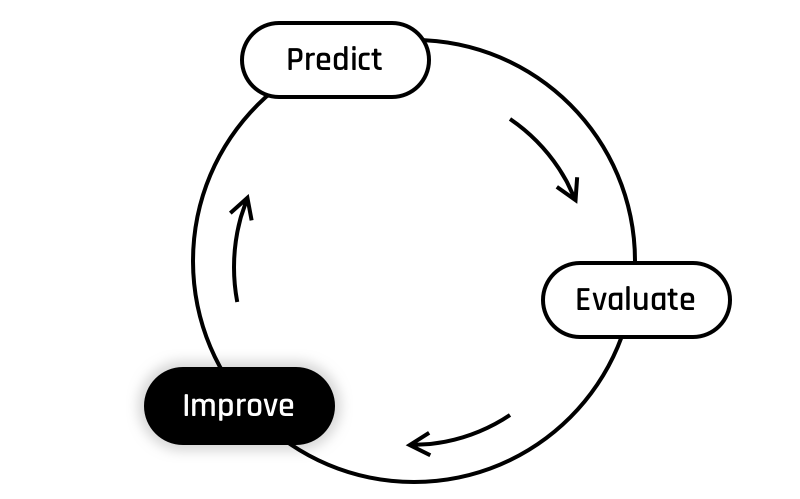
\includegraphics[scale=0.25]{assets/Improve.png}
    %\caption{The Learning Cycle: Improve}
\end{figure}
\noindent{To derive the gradient of the regularized loss function, $\nabla(J)$ 
you have to change a bit the formula of the unregularized gradient.}\\
\\
Given the fact that we are not penalizing $\theta_0$, the formula will remain 
the same as before for this parameter. For the other parameters ($\theta_1, \dots, \theta_n$),
 we must add the partial derivative of the regularization term: $\lambda \theta_j$.\\
\\
Therefore, we get:
$$
\nabla(J)_0 = \frac{1}{m}\sum_{i=1}^{m}(h_\theta(x^{(i)}) - y^{(i)})
$$
$$
\nabla(J)_j = \frac{1}{m}\left(\sum_{i=1}^{m}(h_\theta(x^{(i)}) - y^{(i)})x_j^{(i)} + \lambda \theta_j\right) \text{ for j = 1, ..., n}
$$
\\
Where:  
\begin{itemize}
    \item $\nabla(J)_j$ is the j$^\text{th}$ component of the gradient vector $\nabla(J)$
    \item $m$ is the number of training examples used
    \item $h_\theta(x^{(i)})$ is the model's prediction for the i$^\text{th}$ training example
    \item $x^{(i)}$ is the feature vector of the i$^\text{th}$ training example
    \item $y^{(i)}$ is the expected target value for the i$^\text{th}$ example
    \item $\lambda$ is a constant, the regularization hyperparameter
    \item $\theta_j$ is the j$^\text{th}$ parameter of the $\theta$ vector
\end{itemize}
\bigskip
Which can be vectorized as:
$$
\nabla(J) = \frac{1}{m} [X'^T(h_\theta(X) - y) + \lambda \theta']
$$  
\\
Where:  
\begin{itemize}
    \item $\nabla(J)$ is a vector of length $(n + 1)$, the gradient vector
    \item $m$ is the number of training examples used
    \item $X$ is a matrix of dimension $(m \times n)$, the design matrix
    \item $X'$ is a matrix of dimension $(m \times (n + 1))$, the design matrix onto 
    which a column of ones is added as a first column
    \item $y$ is a vector of length $m$, the vector of expected values
    \item $h_\theta(X)$ is a vector of length $m$, the vector of predicted values
    \item $\lambda$ is a constant
    \item $\theta$ is a vector of length $(n + 1)$, the parameter vector
    \item $\theta'$ is a vector of length $(n + 1)$, constructed using the following rules:
\end{itemize}

$$
\begin{matrix}
\theta'_0 & =  0 \\
\theta'_j & =  \theta_j & \text{ for } j = 1, \dots, n\\    
\end{matrix}
$$

% =============================================== %
\subsection*{Linear Gradient vs Logistic Gradient}
% ----------------------------------------------- %
As before, we draw your attention on the only difference between the linear regression's 
and the logistic regression's gradient equations: \textbf{the hypothesis function} $h_\theta(X)$.
\begin{itemize}
    \item In the linear regression: $h_\theta(X) = X'\theta$
    \item In the logistic regression: $h_\theta(X) = \text{sigmoid}(X'\theta)$
\end{itemize}

\newpage
\turnindir{ex04}
\exnumber{04}
\exfiles{log\_gradient.py}
\exforbidden{any function that performs derivatives for you}
\makeheaderfilesforbidden


% ================================= %
\section*{Objective}
% --------------------------------- %
Understand and manipulate the concept of gradient in the context of logistic formulation.\\
\\
You must implement the following formula as a function:  

$$
\begin{matrix}
\nabla(J)_0 &  = &\cfrac{1}{m}\sum_{i=1}^{m}(h_{\theta}(x^{(i)}) - y^{(i)}) & \\
\nabla(J)_j & = &\cfrac{1}{m}\sum_{i=1}^{m}(h_{\theta}(x^{(i)}) - y^{(i)})x_{j}^{(i)} & \text{ for j = 1, ..., n}    
\end{matrix}
$$
\\
Where:
\begin{itemize}
  \item $\nabla(J)$ is a vector of length $(n + 1)$, the gradient vector
  \item $\nabla(J)_j$ is the j$^\text{th}$ component of $\nabla(J)$, the partial derivative of $J$ with respect to $\theta_j$
  \item $y$ is a vector of length $m$, the vector of expected values
  \item $y^{(i)}$ is a scalar, the i$^\text{th}$ component of vector $y$
  \item $x^{(i)}$ is the feature vector of the i$^\text{th}$ example
  \item $x^{(i)}_j$ is a scalar, the j$^\text{th}$ feature value of the i$^\text{th}$ example
  \item $h_{\theta}(x^{(i)})$ is a scalar, the model's estimation of $y^{(i)}$
\end{itemize}
\bigskip
\noindent{Remember that with logistic regression, the hypothesis is slightly different:}\\
$$
h_{\theta}(x^{(i)}) = sigmoid( \theta \cdot x'^{(i)})
$$
\newpage

% ================================= %
\section*{Instructions}
% --------------------------------- %
In the \texttt{log\_gradient.py} file, write the following function as per the instructions below:\\

\begin{minted}[bgcolor=darcula-back,formatcom=\color{lightgrey},fontsize=\scriptsize]{python}
def log_gradient(x, y, theta):
    """Computes a gradient vector from three non-empty numpy.ndarray, with a for-loop. The three arrays must have compatible dimensions.
    Args:
      x: has to be an numpy.ndarray, a matrix of shape m * n.
      y: has to be an numpy.ndarray, a vector of shape m * 1.
      theta: has to be an numpy.ndarray, a vector of shape (n + 1) * 1.
    Returns:
      The gradient as a numpy.ndarray, a vector of shape n * 1, containing the result of the formula for all j.
      None if x, y, or theta are empty numpy.ndarray.
      None if x, y and theta do not have compatible dimensions.
    Raises:
      This function should not raise any Exception.
    """
    ... Your code ...
\end{minted}

% ================================= %
\section*{Examples}
% ================================= %
\begin{minted}[bgcolor=darcula-back,formatcom=\color{lightgrey},fontsize=\scriptsize]{python}
# Example 1:
y1 = np.array([1]).reshape((-1, 1))
x1 = np.array([4]).reshape((-1, 1))
theta1 = np.array([[2], [0.5]])

log_gradient(x1, y1, theta1)
# Output:
array([[-0.01798621],
       [-0.07194484]])

# Example 2: 
y2 = np.array([[1], [0], [1], [0], [1]])
x2 = np.array([[4], [7.16], [3.2], [9.37], [0.56]])
theta2 = np.array([[2], [0.5]])

log_gradient(x2, y2, theta2)
# Output:
array([[0.3715235 ],
       [3.25647547]])

# Example 3: 
y3 = np.array([[0], [1], [1]])
x3 = np.array([[0, 2, 3, 4], [2, 4, 5, 5], [1, 3, 2, 7]])
theta3 = np.array([[-2.4], [-1.5], [0.3], [-1.4], [0.7]])

log_gradient(x3, y3, theta3)
# Output:
array([[-0.55711039],
       [-0.90334809],
       [-2.01756886],
       [-2.10071291],
       [-3.27257351]])
\end{minted}